\section{Partie 1: Migration de NTMIX en Fortran 90}

Avant de commencer à développer une version en 3 dimensions de NTMIX, j'ai dû moderniser le code. En effet, NTMIX a été développé en Fortran 77 ce qui ne permettait pas l'allocation dynamique de tableau; l'ensemble des variables étaient allouées de manière statique. Pour résoudre ce problème et permettre plus de flexibilité, il m'a été demandé de migrer le code du standard Fortran 77 au standard Fortran 90.
% Le programme devait donc être entièrement recompilé à chaque changement de la taille du maillage.

\subsection{Migration de NTMIX}
\subsubsection{Travail réalisé}

\paragraph{Réécriture de code}Cette partie consistait donc à réécrire le code dans une norme plus récente. Une majorité des modifications était liée à la syntaxe du code. Pour rendre la tâche plus aisée, j'ai utilisé des expressions régulières; ce sont des séquences de caractères qui définissent des motifs de recherche et qui sont particulièrement utiles pour remplacer un motif par un autre. Par exemple, la figure \ref{fig:regex} montre une expression utilisée pour modifier les commentaires dans le code; ils sont très nombreux et on peut donc automatiser la tâche. En Fortran 77, le C ou c placé en début de ligne indique le début d'un commentaire mais en Fortran 90 c'est un ! qui a cet usage.

\begin{figure}[ht]
  \centering
  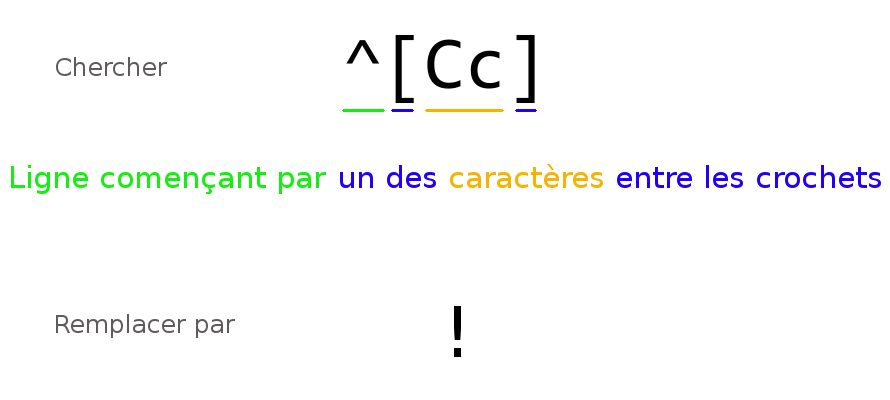
\includegraphics[scale=0.3]{figures/regex.png}
  \caption{\label{fig:regex}Exemple d'expression régulière}
\end{figure}

%Exemple ^#.*?"\(.*?\)\.com"

\paragraph{Gestion de la mémoire}En Fortran, les blocs COMMON permettent de définir des zones mémoires globales, accessible depuis n'importe où dans le code. Le problème est qu'il faut répliquer ce bloc à chaque endroit du code où les variables qu'il contient doivent être utilisées, le plus souvent avec des instructions non-standard du Fortran. Un autre problème est qu'il faut définir la taille des tableaux contenus dans ces blocs à la compilation, ce qu'y va à l'encontre de mon objectif. Pour palier à ces problèmes, ces blocs ont été transformés en modules (introduits en Fortran 90) qui permettent également d'avoir une zone de mémoire globale mais les tailles des tableaux peuvent être précisées à l'exécution.

\paragraph{Post-traitement}NTMIX génère des fichiers binaires contenant l'état physique de la simulation à un instant donnée. Un programme annexe à NTMIX permettait de transformer ces fichiers en fichiers pouvant être visualisés grâce à Plot3D. Ce code ne fonctionnant plus, je l'ai modifié pour qu'il génère des fichiers HDF5 (Hierarchical Data Format) qui permettent de structurer de grandes quantités de données. Cependant, ces fichiers ne peuvent être directement lus par un logiciel de visualisation, j'y ai donc joint des fichiers XDMF (eXtensible Data Model and Format). Ce format a été développé pour le calcul haute performance et notamment pour permettre la visualisation des données par des logiciels comme ParaView ou EnSight en autorisant la définition d'un maillage auquel joindre les données.


\begin{figure}[ht]
  \centering
  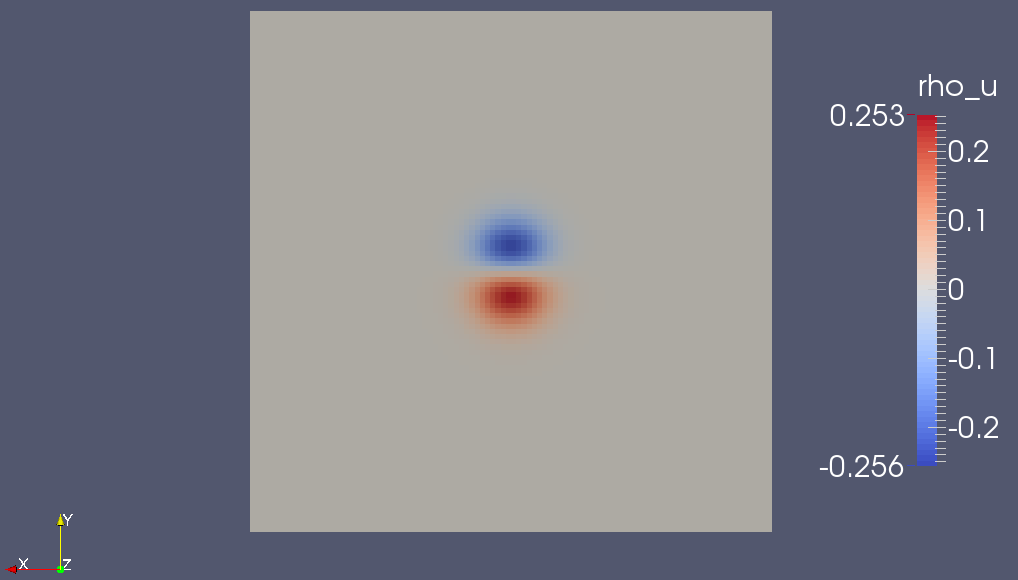
\includegraphics[scale=0.3]{figures/vertex.png}
  \caption{\label{fig:visu}Exemple de visualisation - ParaView}
\end{figure}

%\begin{itemize}
%\item Changement de syntaxe
%\item Changement des bloc commom en modules
%\item Changement des equivalence en pointeur
%\item Allocation dynamique des tableaux
%\item Utilisation de namelist pour changer la taille du maillage et certains paramètres du problème physique.
%\end{itemize}


\subsubsection{Validation}Pour vérifier que les modifications réalisées ne changeaient pas le comportement du programme, j'ai écrit un script permettant de comparer les résultats fournis par ma version avec ceux du programme initial. NTMIX lit la configuration physique de la simulation depuis des fichiers d'entrée. Le script génère donc ces fichiers avec plusieurs configuration, lance la version initiale, la version en cours de développement puis compare les solutions calculées par ceux-ci.




\subsection{Passage en 3D}

\subsubsection{Méthode}\label{sec:3dmeth}
Dans cette partie, je me suis intéressé au passage de l'application en 3 dimensions. Pour minimiser les erreurs pouvant être induites par ce changement, j'ai modifié le code par petits blocs. Une grande partie des variables conservatives (densité, vitesses, énergie..) sont stockées dans un seul tableau et des pointeurs viennent délimiter ce tableau en sous-tableaux (fig. \ref{fig:array_2d}). Ces pointeurs représentaient tous des tableaux 2D. J'ai donc dans un premier temps modifié la taille du grand tableau pour qu'il puisse contenir la dimension supplémentaire mais en laissant les pointeurs aux bon emplacements et j'ai ajouté des tableaux 3D, qui n'étaient pas encore utilisés à ce moment-là. A partir de là, j'ai remplacé progressivement les tableaux 2D par les tableaux 3D en vérifiant que les résultats restaient identiques au fur et à mesure. Cette méthode m'a donc permis de réduire le risque d'erreurs au maximum.

\paragraph{}Après avoir réalisé ces modifications, je me suis intéressé aux calculs des dérivées. Ces dérivées permettent de modifier l'état de la simulation. Maintenant que NTMIX était en 3D, il fallait.

\paragraph{}NSCBC(Navier-Strokes Characteristic Boundary Conditions) demander à bénédicte une explication (waves ?) \cite{POINSOT1992104}

\paragraph{}Plusieurs parties du code prévoyait déjà le passage du code en 3 dimensions, ainsi la préparation du calcul des dérivées était présente et a facilité le travail. La librairie CHEMKIN est adimensionnée ce qui permet d'ajouter une dimension sans avoir à modifier les fonctions de celle-ci.

\begin{itemize}
\item Changement de la taille des tableaux
\item Ajout de la vitesse sur l'axe Z
\item Ajout des conditions limites sur Z
\item Modification du calcul des dérivées
\item Modification du calcul de l'énergie cinétique: $\rho_e = \rho\frac{1}{2}(u^2+v^2+w^2)$
\end{itemize}

\subsubsection{Validation}
Comme dit dans précedemment (sec. \ref{sec:3dmeth}), j'ai d'abord testé le comportement du programme 3D en précisant une dimension nulle ce qui m'a permis de comparer les résultats avec la version 2D. J'ai ensuite mis en place plusieurs tests 3D permettant de valider les calculs réalisés par le programme:

\begin{itemize}
\item Écoulements uniformes: un flux uniforme traverse le domaine selon un axe; le flux étant constant, les dérivées doivent rester nulles et les vitesses ne doivent pas varier
\item Front de flamme(expliquer):
  \begin{itemize}
  \item Vitesse nulle: le front de flamme doit rester statique et un phénomène de diffusion doit être observé (mouvement de molécules d'une région de haute concentration vers une région de faible concentration)
  \item Vitesse non-nulle: en plus du phénomène de diffusion, la convection doit également apparaitre (mouvement de groupe de molécules au sein d'un fluide)
  \end{itemize}
\item Turbulence homogène isotrope
\end{itemize}

\paragraph{Écoulements uniformes}
Comme dit précédemment, les dérivées doivent être nulles dans ce cas, la simulation doit donc rester dans son état initial. Comme on peut le voir sur la figure \ref{fig:uniform_flow}, les vitesses selon les 3 axes sont restées constantes au cours du temps.
 
\begin{figure}[ht]
  \centering
 % \includegraphics[scale=0.3]{figures/uniform_flow.png}
  \caption{\label{fig:uniform_flow}Flot uniforme}
\end{figure}

\paragraph{Front de flamme}
Dans ce cas, le front de flamme est modélisé, au temps $t_0$, par une gaussienne centrée en $x_0$: $f(x,t_0)=e^{\frac{-(x-x_0)^2}{\sigma^2}}$ que nous avons simplifiée en $e^{-(x^2)}$. Pour observer l'effet de diffusion, nous utilisons la fonction dérivée d'une gaussienne: $f(x,t)=\frac{1}{t}e^{fr}$.

\begin{figure}[ht]
  \centering
  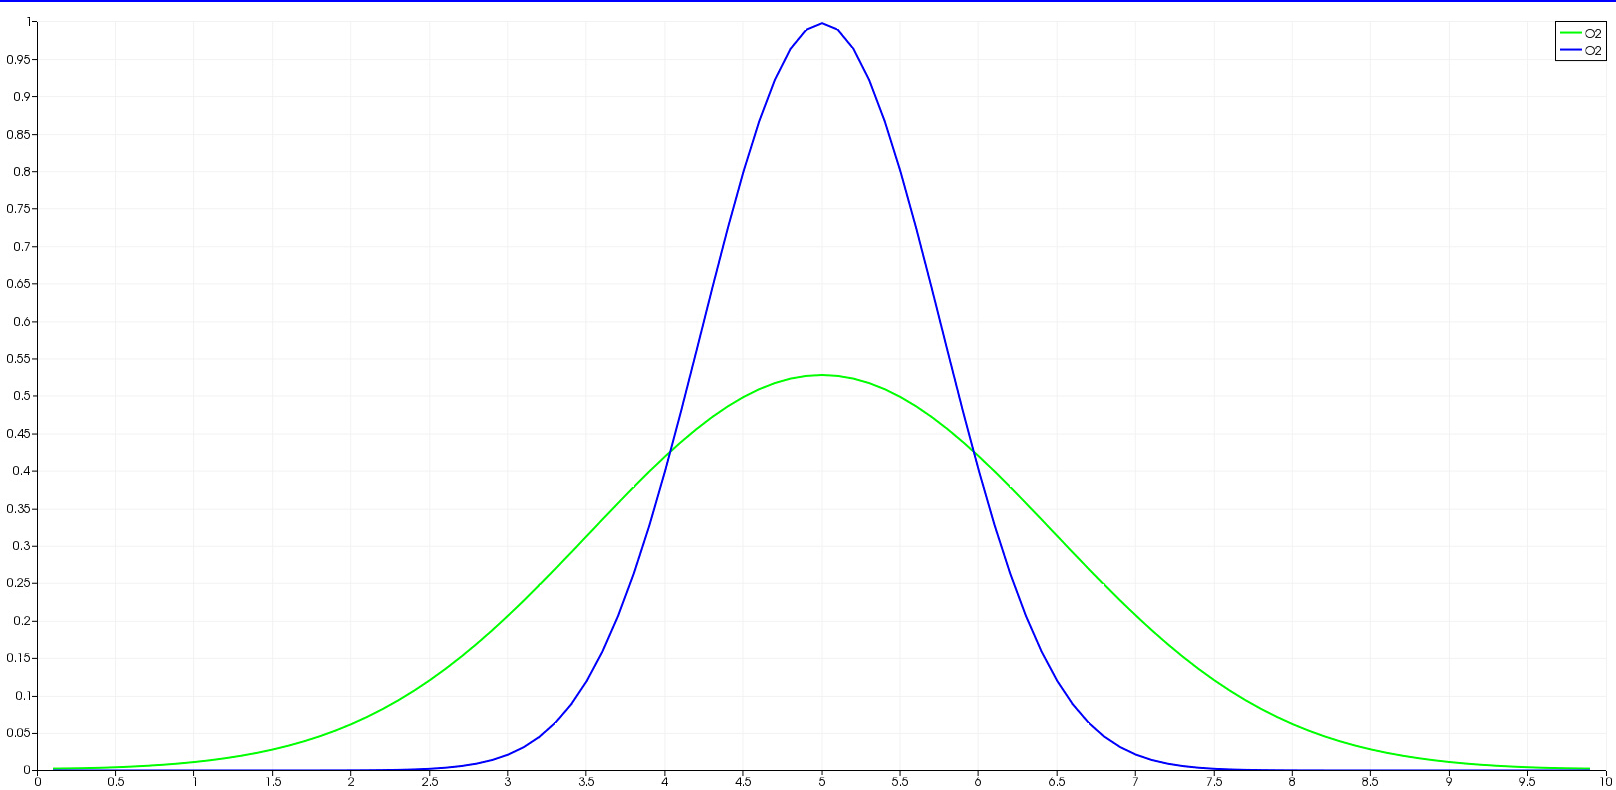
\includegraphics[scale=0.15]{figures/diff.png}
  \caption{\label{fig:diff} }
\end{figure}



\begin{figure}	
  \centering
  \begin{minipage}{.5\textwidth}
    \centering
    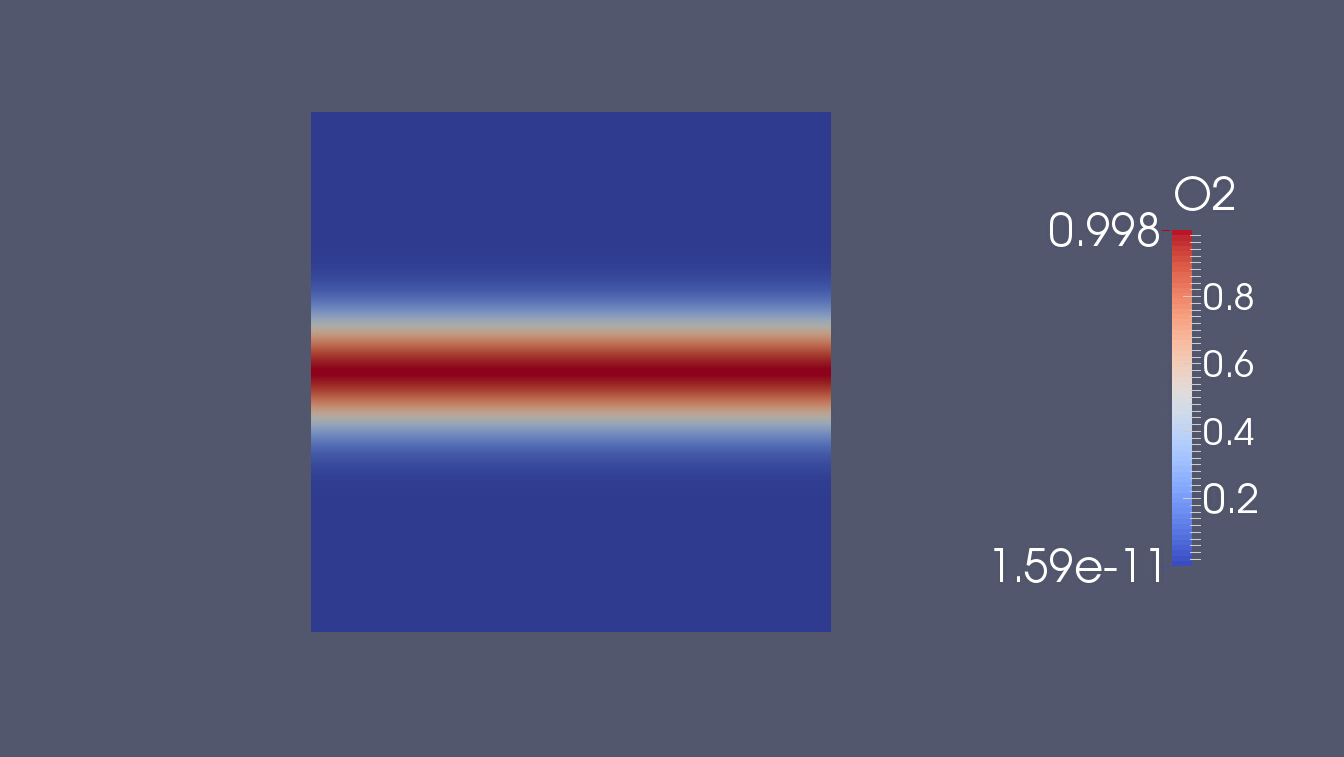
\includegraphics[width=.9\linewidth]{figures/diff_0.png}
    \caption{\label{fig:diff_0}Caption 2}
  \end{minipage}%
  \begin{minipage}{.5\textwidth}
    \centering
    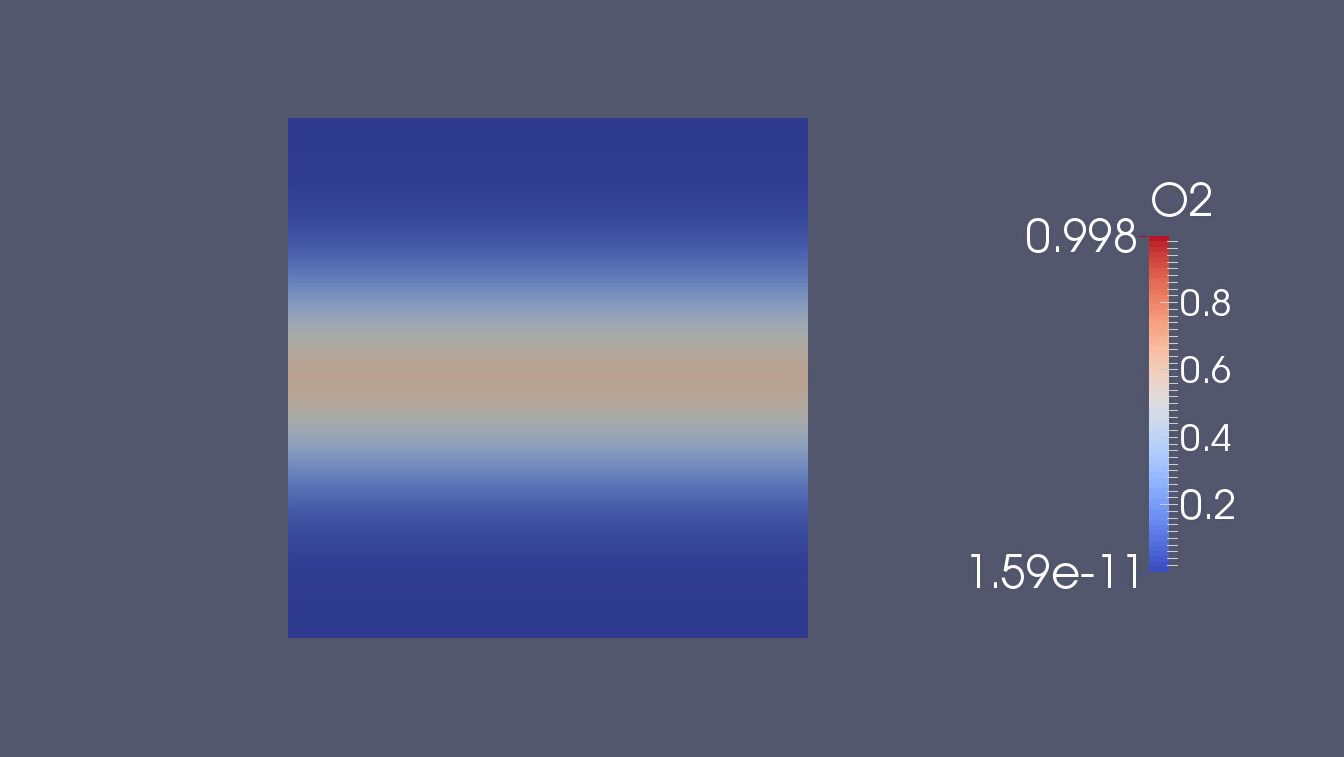
\includegraphics[width=.9\linewidth]{figures/diff_325.png}
    \caption{\label{fig:diff_325}Caption 2}
  \end{minipage}
\end{figure}


\paragraph{Turbulence homogène isotrope}
(help bénédicte)

\begin{figure}[ht]
  \centering
  %\includegraphics[scale=0.3]{figures/turbiso.png}
  \caption{\label{fig:turbiso}Turbulence homogène isotrope}
\end{figure}



